\section{地球系统: 流形上的随机动力学过程}
\label{sec:earth_system}

地球系统是一个典型的\textbf{复杂系统 (Complex System)}，其状态空间维度高，时空尺度跨度大，确定性动力学与随机扰动深度耦合，存在着大量非线性的相互作用与反馈机制 \cite{wang2023earth}。
传统的分析方法和建模方式难以刻画地球系统中发生的各种复杂过程。
因此，我们亟需一套能够同时描述地球系统几何结构与统计特征的理论框架。
基于微分几何，我们提出了一个新的视角: \textbf{将地球系统理解为流形上的随机动力学过程}。

\subsection{时间尺度分离}
\label{sec:timescale_separation}

地球系统跨越从毫秒到百万年的广泛时间尺度 \cite{majda2012climate}。
大气动力调整时间 (声波、重力波) 为分钟至小时，辐射平衡调整为周至月，海洋上层混合为月至年，深海环流为百年至千年，冰盖动力学为千年至万年。
这种时间上的多尺度性质源于系统的能量级联结构和不同物理过程的特征时间差异 \cite{arnold1998random}。
表 \ref{tab:timescales} 列举了主要物理过程及其特征时间。

\begin{table}[htbp]
\centering
\caption{地球系统主要物理过程的特征时间尺度}
\label{tab:timescales}
\begin{tabular}{lcc}
    \hline
    物理过程 & 特征时间 & 主要机制 \\
    \hline
    声波传播 & 秒$\text{--}$分钟 & 压力波动 \\
    重力波、惯性振荡 & 分钟$\text{--}$小时 & 浮力、科氏力 \\
    对流、湍流混合 & 小时$\text{--}$天 & 不稳定增长 \\
    天气系统 (锋面、气旋) & 天$\text{--}$周 & 斜压不稳定 \\
    辐射平衡调整 & 周$\text{--}$月 & 辐射强迫响应 \\
    ENSO、季节内振荡 & 月$\text{--}$年 & 海气耦合 \\
    海洋上层环流 & 年$\text{--}$十年 & 风应力驱动 \\
    深海环流 (AMOC) & 百年$\text{--}$千年 & 热盐环流 \\
    冰盖动力学 & 千年$\text{--}$万年 & 冰流动与消融 \\
    地质构造、火山活动 & 万年$\text{--}$百万年 & 板块运动 \\
    \hline
\end{tabular}
\end{table}

基于这一认识，我们引入\textbf{时间尺度分离假设}:

\begin{assumption}[时间尺度分离]
\label{ass:timescale_separation}
    地球系统的完整状态空间可分解为积空间 $\statespace = \dataspace \times \climatespace$，其中:
    \begin{itemize}
        \item 快变量 (Fast Variables): $\fastvar \in \dataspace \subset \R^N$: 大气温度、气压、风速、湿度、海表温度异常等在短时间尺度 ($\predtime_{\text{fast}} \sim 1$ 天至 $10$ 年) 内显著变化的状态分量;
        \item 慢变量 (Slow Variables): $\slowvar \in \climatespace \subset \R^M$: 大气 $\text{CO}_2$ 浓度、太阳辐射、冰盖体积、地形等在长时间尺度 ($\predtime_{\text{slow}} \sim 10$ 年至 $10^6$ 年) 内缓慢演化的参数。
    \end{itemize}

    假设存在时间尺度分离条件:
    \begin{equation}
    \label{eq:timescale_separation}
        \epsilon = \frac{\predtime_{\text{fast}}}{\predtime_{\text{slow}}} \ll 1
    \end{equation}
\end{assumption}

时间尺度分离为观测时间窗口的选择提供了指导。
当研究天气与短期气候 ($T \leq 10$ 年) 时，可将 $\slowvar$ 视为固定参数，因为慢变量在观测时间窗口内的变化相对于快变量可忽略。
当研究气候变化 ($T \geq 10$ 年) 时，需考虑 $\slowvar(t)$ 的缓慢演化及其对快变量动力学的影响。
两个时间尺度的分界线取决于具体问题，但通常在年际到年代际之间 ($T \sim 1\text{--}10$ 年)。

\subsection{流形假设}
\label{sec:manifold_hypothesis}

快变量 $\fastvar$ 所处的状态空间 $\dataspace = \R^N$ 的维度极高。
考虑 $1^\circ \times 1^\circ$ 网格、30层垂直、6个物理量 (温度、气压、比湿、三维风速)，则 $N = 360 \times 180 \times 30 \times 6 \approx 1.2 \times 10^6$，达到了百万量级。
经典统计学习理论 \cite{vapnik1999nature} 指出，样本复杂度随维度指数增长，即“维度灾难” (Curse of Dimensionality)。
即使我们有几十年的历史观测数据，样本点在如此高维的状态空间中也稀疏得可怜。
因此，理论上我们无法对 $\fastvar$ 进行任何有意义的统计分析。
幸运的是，维度灾难实际上并未阻止我们从事地球系统科学的研究。
其中的关键在于: \textbf{物理上可实现的状态并非均匀分布在整个状态空间 $\dataspace$ 中，而是受到严苛的约束条件，集中在某个低维子集上}。

具体而言，这些约束包括:
\begin{itemize}
    \item \textbf{守恒律}: 质量守恒 $\nabla \cdot (\rho \bm{u}) + \frac{\partial \rho}{\partial t} = 0$，能量守恒，动量守恒——这些约束将状态空间限制在守恒量曲面的交集上；
    \item \textbf{动力学方程}: Navier-Stokes方程、热力学方程、连续性方程——这些方程使得系统的演化受到动力学约束，而非在整个状态空间中任意游走；
    \item \textbf{诊断关系}: 静力平衡 (大尺度运动)、地转平衡 (中高纬度)、状态方程 $p = \rho R T$；
    \item \textbf{边界条件}: 地表边界、大气顶、海陆分布；
    \item \textbf{物理可实现性}: $T, q, p > 0$，相对湿度 $\leq 100\%$，位温随高度变化受静力稳定性约束。
\end{itemize}

在微分几何中，我们称 $\fastvar$ 被约束在一个\textbf{流形 (Manifold)} 上，记作 $\manifold$。
我们不妨假定 $\manifold$ 是光滑的。

\begin{definition}[光滑流形]
\label{def:manifold}
    $\manifolddim$ 维光滑流形 $\manifold$ 是一个拓扑空间，配备图册 $A = \{(U_\alpha, \coordmap_\alpha)\}_{\alpha \in A}$，满足:
    \begin{itemize}
        \item 开覆盖: $\manifold = \bigcup_{\alpha} U_\alpha$；
        \item 局部同胚: 坐标图 $\coordmap_\alpha: U_\alpha \to V_\alpha \subset \R^{\manifolddim}$ 是同胚；
        \item 光滑转移: 转移映射 $\coordmap_\beta \circ \coordmap_\alpha^{-1}$ 是 $C^\infty$ 光滑的。
    \end{itemize}

    流形 $\manifold$ 可嵌入高维空间 $\dataspace$，存在嵌入映射 $\iota: \manifold \hookrightarrow \dataspace$。
\end{definition}

流形是可被“弯曲”但局部“平坦”的子空间，它可以嵌入高维空间，但本身具有较低的内在维度。
在任意点 $p \in \manifold$ 附近的小邻域，流形近似欧氏空间 $\R^{\manifolddim}$，可用 $\manifolddim$ 个坐标参数化。
这一性质是流形区别于分形等更复杂几何结构的关键特征。

\begin{definition}[切空间与流形维度]
\label{def:tangent_space}
    流形 $\manifold$ 在点 $p$ 处的切空间 $T_p\manifold$ 定义为:
    \begin{equation}
    \label{eq:tangent_space}
        T_p\manifold = \{\bm{v} \in \R^N : \bm{v} \perp N_p\manifold\}
    \end{equation}

    其中 $N_p\manifold$ 是法空间。
    $T_p\manifold$ 是由流形在 $p$ 点处的切向量张成的向量空间，是流形在 $p$ 点处的最佳线性逼近。
    流形的维数 $k$ 正是切空间的维数，它度量了流形的内在自由度。
\end{definition}

要想理解流形，我们可以想象一个嵌入在高维空间中的曲面，它可以被弯曲、扭转，但局部总是“平坦”的。
总结刚才的讨论，我们得出了一个深刻的洞察: 尽管观测空间的维度极高，但真实数据的内在自由度却往往很低。
在此基础上，我们提出了\textbf{流形假设 (Manifold Hypothesis)} \cite{fefferman2016testing}:

\begin{assumption}[流形假设]
\label{ass:manifold_hypothesis}
    固定慢变量 $\slowvar$，快变量 $\fastvar$ 嵌入于一个 $\manifolddim$ 维的光滑流形 $\manifold_{\slowvar} \subset \dataspace$ 上，其中 $\manifolddim \ll N$。
\end{assumption}

想象一张“纸”(二维流形) 放在三维空间里 (图 \ref{fig:manifold_hypothesis})。
纸可以弯曲、折叠，但它本质上仍是二维的——你只需要两个坐标 (纸上的横坐标和纵坐标) 就能定位纸上的任意一点，尽管这张纸存在于三维空间中。
这就是“流形假设”: 我们所讨论的地球系统状态场，实际上也就是高维状态空间 $\dataspace$ 中的一张“纸”。

\begin{figure}[htbp]
    \centering
    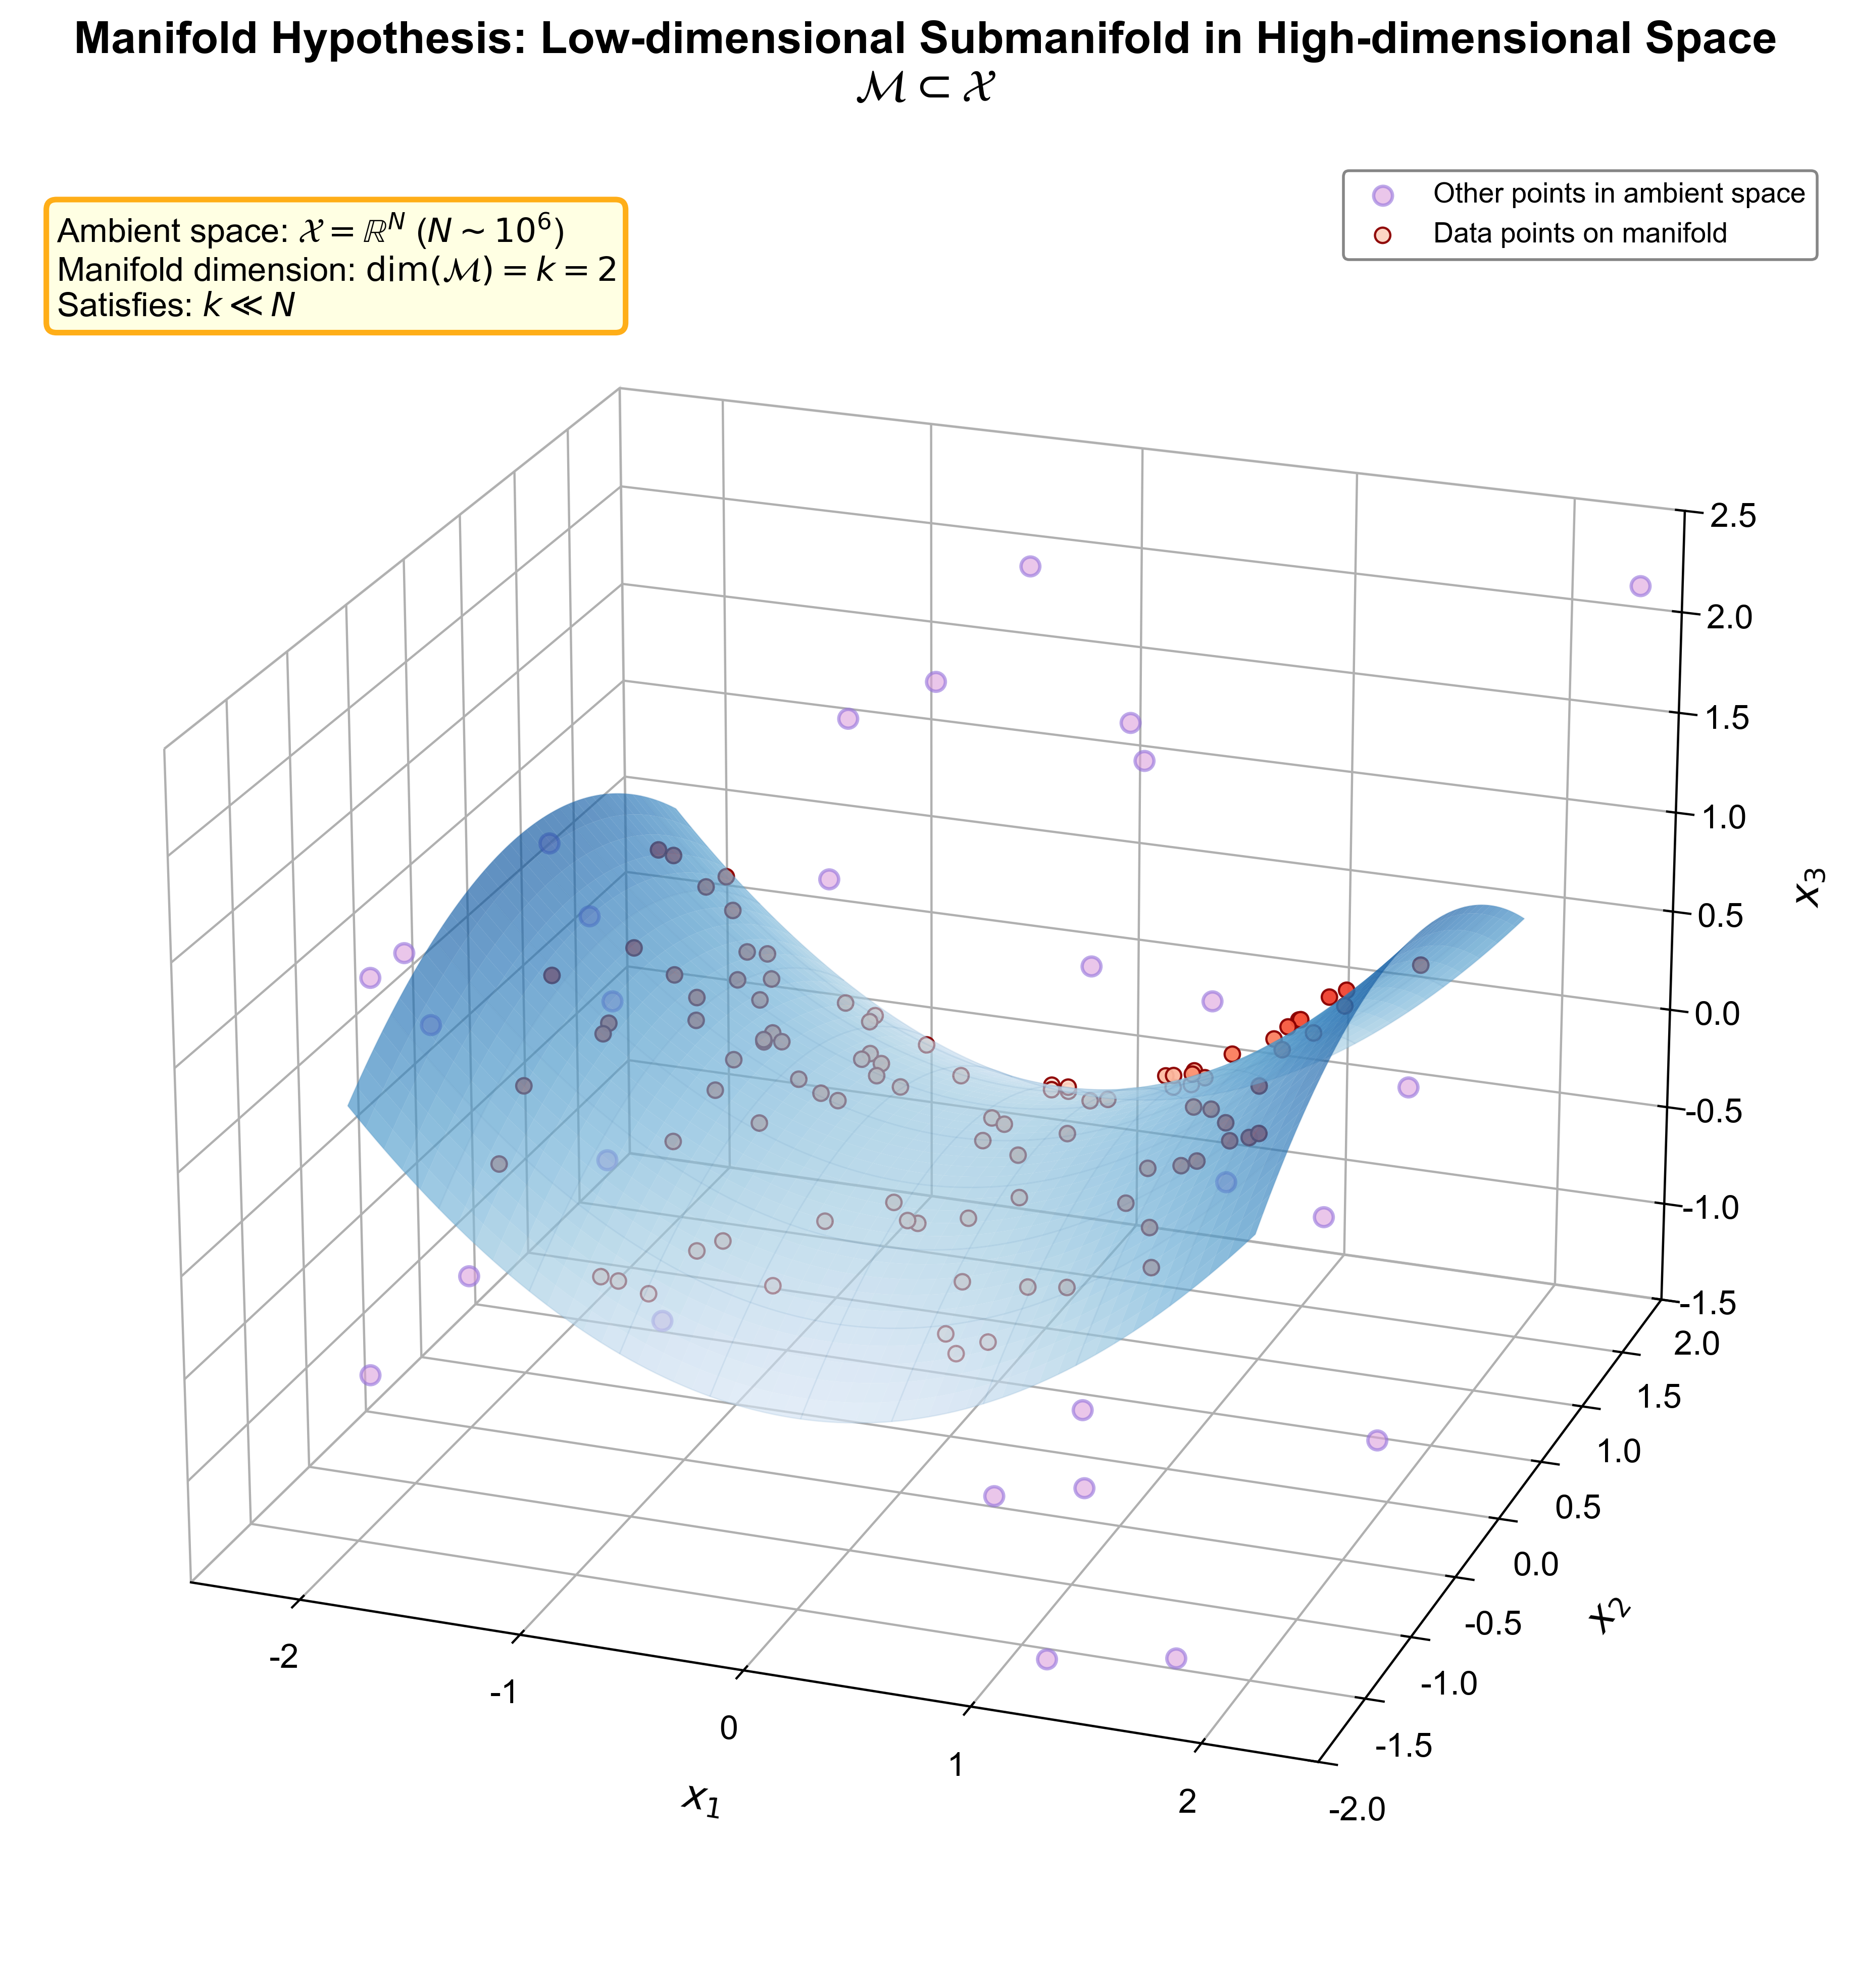
\includegraphics[width=1.00\textwidth]{./assets/manifold_hypothesis.png}
    \caption{流形假设的几何图景。红色点代表观测数据，集中在蓝色曲面 (流形 $\manifold$) 上。紫色点代表环境空间 $\dataspace$ 中的其他点，不在流形上，对应物理上不可实现的状态。}
    \label{fig:manifold_hypothesis}
\end{figure}

经验正交函数 (EOF) 是气候学中最常用的降维方法 \cite{hasselmann1988pips}。
对协方差矩阵 $\bm{C} = \frac{1}{n}\sum_{i=1}^n (\fastvar_i - \bar{\fastvar})(\fastvar_i - \bar{\fastvar})^\top$ 进行特征值分解，前 $K$ 个主成分的累积方差贡献率为:
\begin{equation}
\label{eq:eof_variance_contribution}
    r_K = \frac{\sum_{i=1}^K \eigenval_i}{\sum_{i=1}^N \eigenval_i}
\end{equation}

对于全球大气场，研究发现当 $K \sim 100$ 时，$r_K > 90\%$ \cite{hasselmann1988pips}。
这暗示大气子流形的内在维度约为 $10^2\text{--}10^3$，远小于 $N \sim 10^6$。
对于海洋子流形，主成分对应于一些气候模态: ENSO (解释约40\%方差) \cite{trenberth1997definition}、北大西洋涛动NAO \cite{hurrell1995decadal}、太平洋年代际振荡PDO、北极涛动AO等。
这些模态实际上就是流形的“坐标轴”，它们张成了切空间 $T_p\manifold$，定义了流形在该点的内在几何结构。
不同模态之间的正交性反映了流形局部坐标系的正交选取。

EOF 的有效性验证了流形假设: 如果数据分布在低维流形上，协方差矩阵的秩将远小于 $N$，特征值将快速衰减。
前 $K$ 个主成分对应于流形的坐标方向，任意状态可近似表示为 $\fastvar \approx \bar{\fastvar} + \sum_{k=1}^K a_k \mode_k$，其中 $\{\mode_k\}$ 是主成分，$\{a_k\}$ 是模态系数。

从动力学角度看，物理约束通过快速调整过程持续将状态轨迹“拉回”流形 \cite{ghil2008climate}。
如果因为某种原因产生了偏离流形的状态 (如负湿度、非地转平衡)，快速调整过程 (声波、重力波、湍流混合) 会在短时间内将系统恢复至流形上。
因此，流形具有吸引性，它是动力系统演化的不变集。

慢变量 $\slowvar$ 改变时，约束本身发生变化，流形 $\manifold_{\slowvar}$ 将随之变化。
例如，$\text{CO}_2$ 的增加将改变辐射平衡，温度上升将导致饱和水汽压增加 (Clausius-Clapeyron 关系)，从而改变湿度的可实现范围。
这体现为流形在相空间中的“移动”或“变形”。
在极端情况下，流形的拓扑结构可能会发生突变。

\subsection{参数化随机动力学}
\label{sec:stochastic_dynamics}

在固定慢变量 $\slowvar$ 下，快变量 $\fastvar_t$ 的演化并不是确定性的。
受计算资源限制和观测不确定性的影响，次网格过程 (湍流、对流、云微物理等) 无法被精确模拟，只能使用参数化方案进行统计性描述。
因此，我们需要一个随机动力学框架来描述快变量的演化。

\begin{assumption}[参数化随机动力学]
\label{ass:stochastic_dynamics}
    快变量 $\fastvar_t \in \manifold$ 的演化遵循伊藤随机微分方程 (Itô SDE) \cite{pavliotis2014stochastic}:
    \begin{equation}
    \label{eq:sde}
        d\fastvar_t = \drift(\fastvar_t; \slowvar)\,dt + \diffop(\fastvar_t; \slowvar)\,d\wiener_t
    \end{equation}

    其中:
    \begin{itemize}
        \item $\drift: \manifold \to T\manifold$ 是漂移向量场 (Drift Vector Field)，描述可解析尺度的确定性动力学；
        \item $\wiener_t \in \R^d$ 是 $d$ 维标准维纳过程 (Wiener Process)，满足 $\E[d\wiener_t] = 0$，$\E[d\wiener_t d\wiener_t^\top] = I_d\,dt$；
        \item $\diffop: \manifold \to \mathcal{L}(\R^d, T\manifold)$ 是扩散算子 (Diffusion Operator)，将 $\wiener_t$ 线性映射为切空间中的随机扰动；
        \item $\difftensor(\fastvar; \slowvar) = \diffop(\fastvar; \slowvar)\diffop(\fastvar; \slowvar)^\top \in \R^{N \times N}$ 是扩散张量 (Diffusion Tensor)，对称正定，描述随机扰动的协方差结构。
    \end{itemize}
\end{assumption}

我们逐个解释 Itô SDE 中各项的物理意义 (参见图 \ref{fig:ito_sde}):

\begin{figure}[htbp]
    \centering
    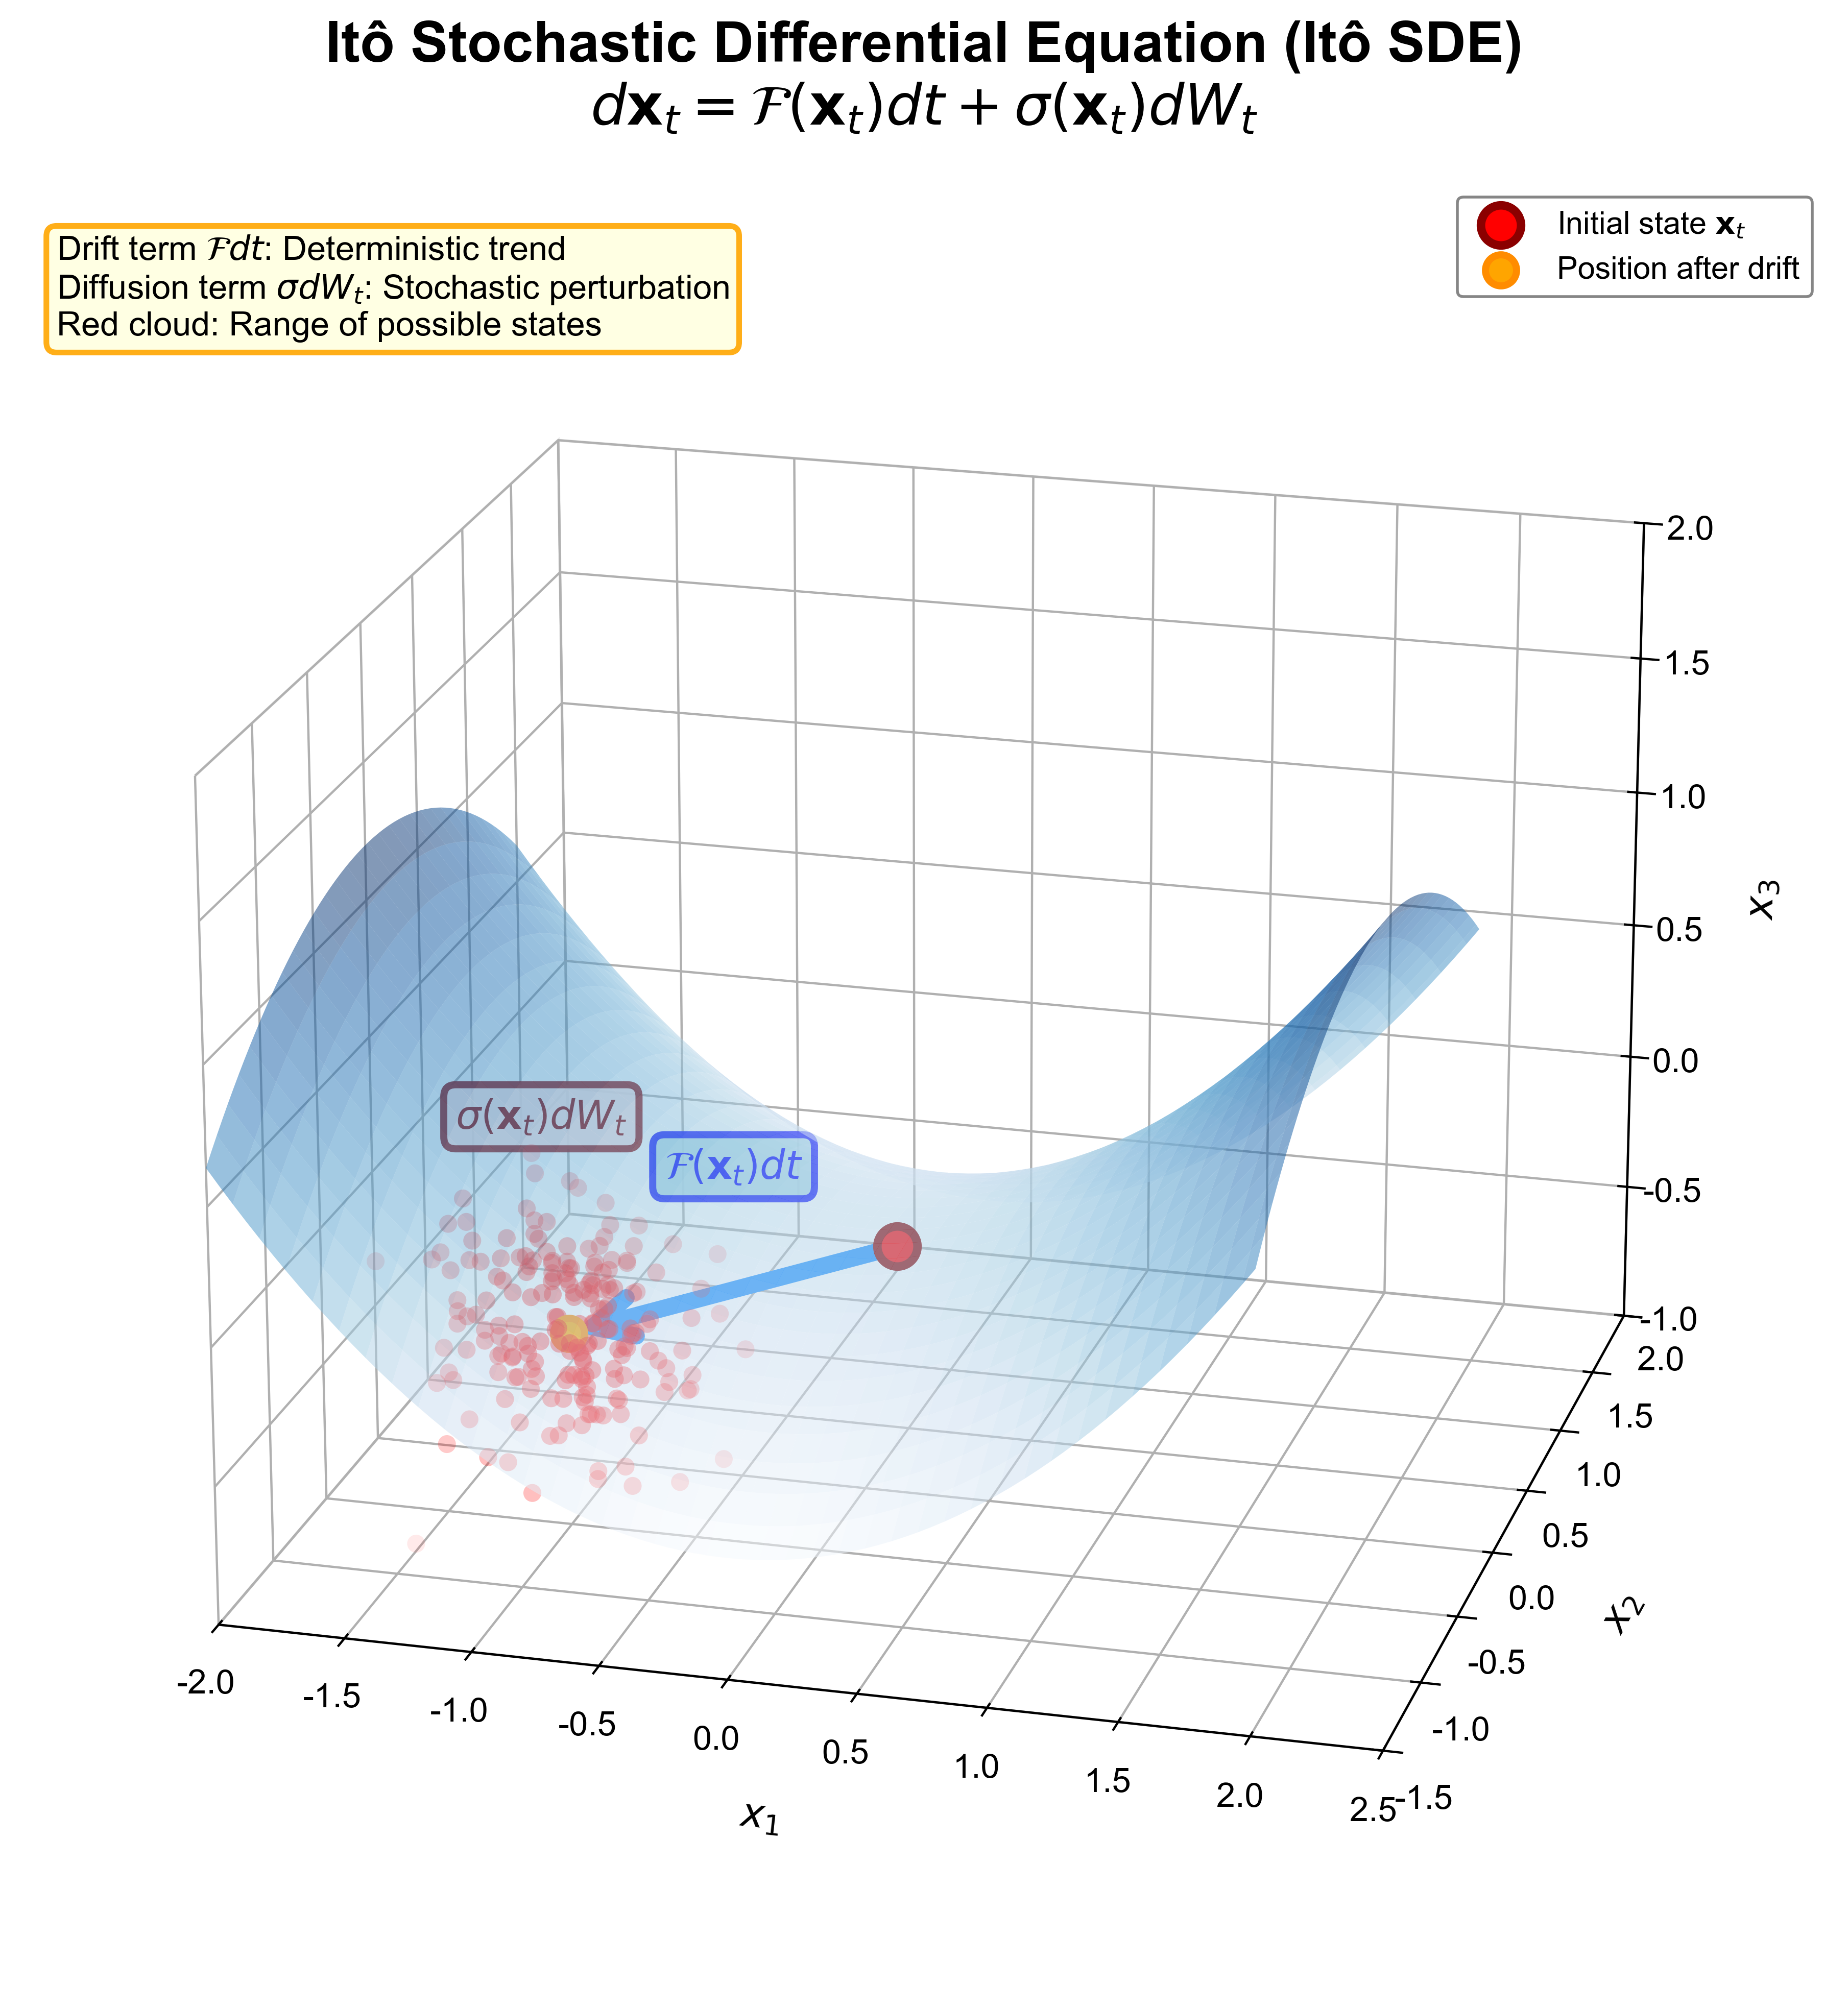
\includegraphics[width=1.00\textwidth]{./assets/ito_sde_visualization.png}
    \caption{伊藤随机微分方程的几何图景。红色点为初始状态 $\fastvar_t$，蓝色箭头为确定性漂移 $\drift(\fastvar_t)dt$，红色云团为随机扩散 $\diffop(\fastvar_t)d\wiener_t$ 产生的可能状态范围。橙色点为经过漂移后的状态。}
    \label{fig:ito_sde}
\end{figure}

\textbf{(1) 漂移项 $\drift(\fastvar; \slowvar)$}: 表示网格尺度可解析的物理过程，以及通过参数化方案统计性解析的次网格过程的系统性影响。
例如，在大气模式中，漂移项包括辐射强迫、大尺度平流、地转风平衡等确定性过程，也包括对流参数化方案给出的平均加热率、湍流参数化方案给出的平均应力。
在海洋模式中，漂移项包括风应力驱动的环流、温盐环流、以及涡参数化方案给出的平均输送。

\textbf{(2) 扩散项 $\diffop(\fastvar; \slowvar)\,d\wiener_t$}: 表示次网格过程的随机波动。
单个对流单体、湍流涡旋的生消是混沌的，无法显式跟踪。
在排除系统性影响 (已体现在漂移项) 后，我们可以用随机扩散描述其概率分布。
扩散张量 $\difftensor(\fastvar; \slowvar)$ 的对角元 $\difftensor_{ii}$ 表示第 $i$ 个自由度的随机扰动强度，非对角元 $\difftensor_{ij}$ 表示不同自由度的随机扰动相关性。
$\difftensor$ 的特征值和特征向量反映了随机扰动的主方向和强度。

\textbf{(3) 维纳过程的维度 $d$}: $d$ 是独立随机源的数量，可理解为主导的随机模态数 (如不同波数的湍流模态)。
扩散算子 $\diffop \in \R^{N \times d}$ 将 $d$ 维随机源映射为 $N$ 维状态扰动，通常 $d \ll N$。
这意味着随机扰动同样具有低维结构: 虽然状态空间是高维的，但驱动随机性的独立源数量有限。

方程 \eqref{eq:sde} 定义了一个马尔可夫过程 (Markov Process): 未来演化只依赖当前状态 $\fastvar_t$，与过去路径无关。
这假定了扩散项的记忆时间远小于漂移项的演化时间，即认为随机扰动无自相关 (白噪声近似)。
物理上，这要求次网格过程的相关时间 (湍流涡旋的寿命、对流单体的持续时间) 远小于大尺度演化的特征时间。
对于大气湍流 ($\sim$ 分钟)，相对于天气系统 ($\sim$ 天)，这一假设是合理的。
但对于某些中尺度过程 (如对流组织化)，可能需要考虑记忆效应，引入分数布朗运动、记忆核等非马尔可夫模型。

\vspace{1em}

我们建立的描述地球系统演化的随机动力学框架与Hasselmann \cite{hasselmann1976stochastic} 的开创性工作有着深刻的联系。
Hasselmann最早提出，快变量 (如大气湍流、对流) 对慢变量 (如海表温度) 的影响可以分解为两部分: 系统性的平均效应和随机的涨落效应。
他以此为基础构建了随机气候模型，成功解释了气候系统的红噪声谱特征，即气候变率的能量集中在低频段 \cite{hasselmann1976stochastic}。

然而，Hasselmann的原始工作主要基于物理直觉，缺乏严格的数学框架。
而现在，通过时间尺度分离、流形假设、Itô SDE等工具，我们可以将Hasselmann的随机气候模型纳入一个统一、严格的数学框架中。
方程 \eqref{eq:sde} 的漂移项 $\drift(\fastvar; \slowvar)$ 即对应于Hasselmann模型中的平均效应，扩散项 $\diffop(\fastvar; \slowvar)\,d\wiener_t$ 则对应于随机涨落。
更重要的是，我们明确了状态空间的流形结构 $\manifold$，将Hasselmann的线性随机模型推广到了非线性流形上，从而可以描述地球系统的几何结构。
